% LAB 2: Basic Loops and Functions
%
% CSE/IT 107: Introduction to Programming
% New Mexico Tech
%
% Prepared by Russell White and Christopher Koch
% Fall 2014
\documentclass[11pt]{cselabheader}

%%%%%%%%%%%%%%%%%% SET TITLES %%%%%%%%%%%%%%%%%%%%%%%%%
\fancyhead[R]{Lab 2: Basic Loops and Functions}
\title{Lab 2: Basic Loops and Functions}

\begin{document}

\pagenumbering{roman}
\maketitle

\begin{figure}[H]
  \centering
  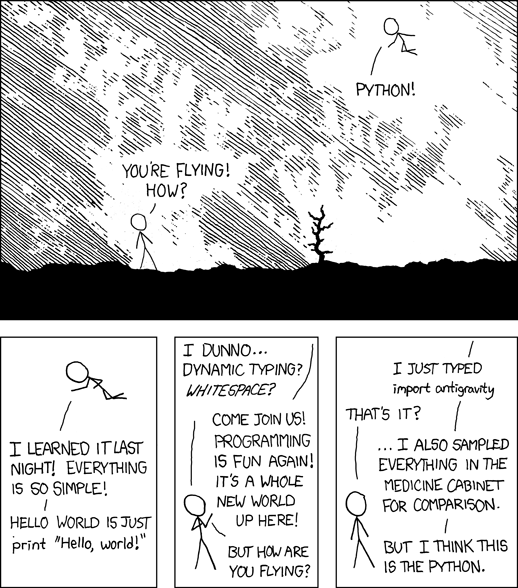
\includegraphics[width=0.85\textwidth]{img/xkcd_python.png}
  \caption{xkcd 353: Python (Source: \url{http://xkcd.com/353})}
\end{figure}

\pagebreak
\thispagestyle{empty}
\hrule
\begin{quotation}
``Only ugly languages become popular. Python is the exception.''
\end{quotation}
\begin{flushright}
  --- Donald Knuth
\end{flushright}

\begin{quotation}
``Simplicity is the ultimate sophistication.''
\end{quotation}
\begin{flushright}
--- Leonardo Da Vinci
\end{flushright}

\begin{quotation}
``How do we convince people that in programming simplicity and clarity -- in
short: what mathematicians call elegance -- are not a dispensable luxury, but
a crucial matter that decides between success and failure?''
\end{quotation}
\begin{flushright}
--- Edsger Dijkstra
\end{flushright}

\hrule

\section{Introduction}
\addcontentsline{toc}{section}{Introduction}

The purpose of this lab is to expand upon the fundamentals of flow control.
In the previous lab, we showed you how to do basic calculations in Python,
like converting temperature from Celsius to Fahrenheit and Kelvin, as well
as using \pythoninline!if!, \pythoninline!elif!, and \pythoninline!else! to
execute different code depending on what values are given to the program.

In some of the exercises (like \pythoninline!star.py!), you likely needed to
repeat lines of code in order to draw your shape correctly. Hopefully this struck
you as something that would be nice to avoid: it might be sustainable with fairly
simple shapes, but what if you wanted a 100-pointed star? Or what if you wanted to
have the user type in a number to determine how many sides they wanted their shape
to have? Clearly, repeating lines of code is not sustainable. In this lab, you will
learn about the \pythoninline!while! statement to help with code you want to run
several times.

We will also be learning about functions, which allow you to group your code
into conveniently reusable chunks.

\pagebreak

\tableofcontents

\pagebreak

\pagenumbering{arabic}
\section{On Types}

In Python, every value has a type.
% In Python, every value is associated with what we call a type.
We have already
seen a few types in action: integers, floating-point numbers, strings, and
boolean values.
The type of a value or variable restricts what it can represent.
Here is a list of some types and example values.

% The type of a value restricts the set of things that it can
% represent.

% An integer can be any whole number, for example \pythoninline{5}. A
% float (floating-point number) is a number with decimal places, for example
% \pythoninline{3.14} or \pythoninline{5.0}. A string is a sequence of characters
% (letters, numbers, \ldots) enclosed by either double or single quotes, for
% example \pythoninline{"I'm a string!"}. A boolean, as we just learned, can have
% two values: \pythoninline{True} or \pythoninline{False}.

\begin{center}
\begin{tabular}{llll}
Name & Description & Examples & Try to cast \pythoninline{y} to this type
\\
\midrule
\texttt{int} & Integer,  whole number & \pythoninline{1, 123, -12, }\dots & \pythoninline{int(y)}
\\
\texttt{float} & Floating-point number & \pythoninline{1.0, 3.1415, -0.01, }\dots & \pythoninline{float(y)}
\\
\texttt{string} & Sequence of characters & \pythoninline{"",  "1",  "abc 123\n", }\dots & \pythoninline{str(y)}
\\
\texttt{boolean} & True or false & \pythoninline{True,  False} & \pythoninline{bool(y)}
\\
\end{tabular}
\end{center}

Most programming languages have types for a good reason: for one, operations
(such as \pythoninline{+}, \pythoninline{-}, \ldots) have different effects on
different types. For example, an integer \pythoninline{*} an integer results in
an integer (the multiplication of the two \emph{operands}), but an integer
\pythoninline{*} a string results in the string repeated. However, a string
\pythoninline{*} a string results in an error:
\begin{pyconcode}
>>> 5*3
15
>>> 5*'hi'
'hihihihihi'
>>> 'hi'*'hi'
Traceback (most recent call last):
  File "<stdin>", line 1, in <module>
TypeError: can't multiply sequence by non-int of type 'str'
\end{pyconcode}

In addition to that, some operations do not work on some types, which helps
ensure correctness of your program.

Also, Python can speed up your programs by picking efficient ways of dealing with different types.
Multiplying integers and multiplying floating point numbers require very different techniques.
Knowing what kind of number is being used, Python can optimize that code.
% Also, depending on the type of the operands,
% Python has different implementations of what goes on under the hood, which can
% then be optimized for each type separately.

% Of course, there are ways to convert between types and there are ways to find
% out what type the value of a specific variable is.
\subsection{The \protect\pythoninline{type()} Function}
Use the function \pythoninline{type()} to find out the type of a value or the
type of the value of a specific variable.

\begin{pyconcode}
>>> type(5)
<class 'int'>
>>> x = 10
>>> type(x)
<class 'int'>
>>> x = 'Allons-y!'
>>> type(x)
<class 'str'>
>>> type(True)
<class 'bool'>
>>> x = "5.5" # string containing 5.5
>>> y = float("5.5") # convert string with 5.5 to a float
>>> y
5.5
>>> z = int("5") # integer containing 5
>>> z
5
>>> q = str(5) # string containing 5
>>> q
'5'
>>> # Note that an impossible conversion will throw an error
>>> int("55a")
Traceback (most recent call last):
  File "<stdin>", line 1, in <module>
ValueError: invalid literal for int() with base 10: '55a'
\end{pyconcode}

\subsection{Casting}
We call the process of converting a value from one type to another type
\emph{casting}. Note that only values have types, and variables can hold
different values.  Applying \pythoninline{type()} to a variable will give you
the type of the value that it holds at the time. In the previous section, we
learned about comparison operators such as \pythoninline{!=}, \pythoninline{<},
\pythoninline{>}, etc. What was not mentioned is that these comparison operators
also compare the type in some cases, but not in others:
\begin{pyconcode}
>>> 5.5 == '5.5' # comparing a string to a float does not work
False
>>> x = 5.5
>>> y = 5.5
>>> x == y
True
>>> 5.5 == float('5.5')
True
>>> 5.0 == 5 # comparing a float and an int works
True
\end{pyconcode}

The usual rule for what works and what does not work with comparisons is to
listen to your intuition: it makes sense to compare different types of numbers;
while it does not make sense to compare strings with numbers.

\subsection{Summary}

\begin{itemize}
  \item A type is a set of values that it can represent.
  \item Casting is the process of converting a value from one type to another.
  \item To find out what type a value / variable is, use the
    \pythoninline{type()} function.
  \item Types we know about at this point:
        \pythoninline{str}, \pythoninline{int}, \pythoninline{float}, \pythoninline{bool}
  \item Not coincidentally, these type names are also the names of the casting
    functions.
  % \item Types we know about at this point:
  %   \begin{multicols}{2}
  %     \begin{itemize}
  %       \item \pythoninline{str} -- string
  %       \item \pythoninline{int} -- integer number
  %       \item \pythoninline{float} -- floating-point number
  %       \item \pythoninline{bool} -- boolean value
  %     \end{itemize}
  %   \end{multicols}
  %   Not coincidentally, these type names are also the names of the casting
  %   functions.
\end{itemize}

\pagebreak
\section{Signaling Errors with \protect\pythoninline{assert}}
The built-in function \pythoninline{assert} can be used to ensure a
condition is true.
If the condition is false, the program is supposed to crash.
To be precise, an \pythoninline{AssertionError} exception is raised
(we will learn more about exceptions in later lessons.)
Here's an example:
\begin{pyconcode}
>>> assert(True)
>>> assert(False)
Traceback (most recent call last):
  File ``<stdin>'', line 1, in <module>
AssertionError
>>> should_be_positive = 1
>>> assert(should_be_positive > 0)
>>> should_be_positive = -1
>>> assert(should_be_positive > 0)
Traceback (most recent call last):
  File ``<stdin>'', line 1, in <module>
AssertionError
\end{pyconcode}

Consider using \pythoninline{assert} to
\begin{itemize}
\item check parameters are of the correct type
\item check for ``can't happen'' situations
\item verify invariants in your code
\item make sure a called function's return value is reasonable.
\end{itemize}

\section{Making Calculations Shorter}
\label{sec:calc}

We showed you simple Python operators such as \pythoninline{+},
\pythoninline{-}, \pythoninline{*}, \pythoninline{%},
etc in lab 1. There is a small extension to these that you can use to update a
variable:

\begin{pyconcode}
>>> x = 5
>>> x += 3 # same as x = x + 3
>>> x
8
\end{pyconcode}

The available assignment operators are:
\begin{multicols}{2}
\begin{itemize}
  \item \pythoninline{+=} -- addition
  \item \pythoninline{-=} -- subtraction
  \item \pythoninline{*=} -- multiplication
  \item \pythoninline{/=} -- division
  \item \pythoninline{//=} -- integer division
  \item \pythoninline{%=} -- remainder
  \item \pythoninline{**=} -- exponentiation
\end{itemize}
\end{multicols}


\pagebreak
\section{Formatting Strings with \protect\pythoninline{.format()}}

Previously, when we wanted to print out both a number and a string, we
had to resort to this:

\begin{pyconcode}
>>> x = 5
>>> print("x is equal to " + str(x))
x is equal to 5
\end{pyconcode}

However, there is an easier way to accomplish the same thing. By using the
\pythoninline!.format()! command, as shown below, we can have far more options for
how we format our output.
With this we do not need to add a gap in the string and then use \pythoninline{+}.

\begin{pyconcode}
>>> x = 5
>>> print("x is equal to {}".format(x))
x is equal to 5
\end{pyconcode}

% Rather than leaving a gap in our string and then using \pythoninline{+} to add on
% our variable, we instead include \pythoninline!{}! where we wish to place our
% variable and add on \pythoninline{.format(x)} to the end of the string.
This
replaces \pythoninline!{}! with the value of \pythoninline{x}.
If we include multiple instances of \pythoninline!{}! in our string, we can then
pass multiple variables to \pythoninline{.format()}. It will place them in the
string in the order provided.

\begin{pyconcode}
>>> x = 5
>>> y = 6
>>> print("x is equal to {} and y is equal to {}.".format(x, y))
x is equal to 5 and y is equal to 6.
\end{pyconcode}

We can also use \pythoninline!.format()! to control our output. For example, we
can restrict how many decimal places a floating point number is printed with. To
do this, we add \pythoninline{:.2f} inside of the \pythoninline!{}!. The
\pythoninline{.2f} specifies that we want 2 digits to follow the decimal point.
%If we wanted to, we
%could add an extra number before the colon to specify which of the arguments we
%want in this position. We don't want to mess with the order of the arguments, so
%we leave the position before the colon blank.

\begin{pyconcode}
>>> print(3.141592653589793)
3.141592653589793
>>> print("{:.2f}".format(3.141592653589793))
3.14
\end{pyconcode}

For more format options, see \url{https://pyformat.info/} and
\begin{center}
  \vspace{-2mm}
  \url{https://docs.python.org/3/library/string.html#format-string-syntax}
  \vspace{-2mm}
\end{center}

\subsection{Summary}

\begin{itemize}
  \item Syntax:
    \begin{python3code}
print("string containing {}".format(variable))
    \end{python3code}

    This will replace the \pythoninline!{}! with the value of
    \pythoninline{variable}.

  \item You can include multiple \pythoninline!{}! in a string and pass multiple
    values to \pythoninline{.format()}.

  \item You can specify advanced formatting options, such as number of digits
    after the decimal point.
\end{itemize}

\pagebreak
\section{Loops}
%Apply the above to while loops.

\subsection{While Loops}
The syntax of a \pythoninline{while} loop is very similar to that of an
\pythoninline{if} statement, but instead of only running the indented block of code
once, the \pythoninline{while} loop will continue running it until the given
boolean statement is no longer true.

\begin{python3code}
x = 10
while x > 0:
    print(x)
    x = x - 1
\end{python3code}

The above program will print out the numbers 10 to 1. Try stepping through this
program on paper, writing out the value of \pythoninline{x} at each time through
the loop. Then repeat for this modified version of the program:

\begin{python3code}
x = 10
while x > 0:
    x = x - 1
    print(x)
\end{python3code}

This version of the program will print out the numbers 9 to 0. This might seem a
bit strange, since the condition of the loop says it will stop when
\pythoninline{x} is no longer larger than 0. And yet, it prints out the value 0
before the loop ends. This is because the loop condition is only checked
whenever the end of the indented section is reached. If the condition is
\pythoninline{True}, then the indented section will be executed again. If the
condition is \pythoninline{False}, then the loop will end.

If the condition starts out \pythoninline{False}, then the loop will never execute.
The following program will not print anything:

\begin{python3code}
x = 0
while x > 0:
    x = x - 1
    print(x)
\end{python3code}

\pythoninline{if} and \pythoninline{else} can be nested within
\pythoninline{while}, as shown below:

\begin{python3code}
x = 10
while x > 0:
    if x % 2 == 0:
        print("{} is even.".format(x))
    else:
        print("{} is odd.".format(x))
    x = x - 1
\end{python3code}

% Of course, they can be nested the other way around, too, with a
They can be nested the other way around, too, with a
\pythoninline!while! inside conditional statements.

Here's an easy way to start an infinite loop:
% There can also be infinite while loops. Try the following:
\begin{python3code}
while True:
    print("Printing forever")
\end{python3code}

Press \emph{Ctrl+C} to stop this loop.

%\subsection{For Loops}
%
%Instead of using \pythoninline!while! loops, you can also use the \pythoninline!for!
%iterator (often also called \pythoninline!for! loop). The \pythoninline!for! loop
%allows you to ``iterate'' over a given list of things, for example a list of
%characters (a string):
%
%\begin{python3code}
%for c in "abc":
%    print("Hi, {}!".format(c))
%\end{python3code}
%
%Here, \pythoninline!c! is a variable you can use inside the code block of the
%for loop.
%
%The example will print:
%
%\begin{verbatimcode}
%Hi, a!
%Hi, b!
%Hi, c!
%\end{verbatimcode}
%
%A for loop can be over numbers as well, but this requires us to use the
%\pythoninline!range()! function. You can give \pythoninline!range()! a starting number
%and an end number:
%
%\begin{python3code}
%for num in range(0, 10):
%    print(num)
%\end{python3code}
%
%This will print the numbers from \emph{zero} to \emph{nine}. Notice that 10 is
%not included!
%
%You can also give \pythoninline!range()! a starting number, an end number, and an
%increment. The increment can be positive or negative. The numbers do not have to
%be actual numbers, you can give variables to it, too:
%
%\begin{python3code}
%start = 10
%end = 0
%increment = -2
%for number in range(start, end, increment):
%    print(number)
%\end{python3code}
%
%This will print:
%
%\begin{verbatimcode}
%10
%8
%6
%4
%2
%\end{verbatimcode}
%
%Notice how zero is not included. The end number is never included when you use
%\pythoninline!range()!.
%
%You can also just have the \pythoninline!for! loop ``iterate'' over a list of
%things:
%
%\begin{python3code}
%for number in [0, -2, 20, 24]:
%    print(number)
%\end{python3code}

\subsection{Nesting}

You can nest loops and conditional statements in any way you
like. The following is just an example:

\begin{python3code}
inputs = 0
while inputs < 10:
    parity = input("Even or odd? ")

    # prints even or odd numbers between 0 and 10, depending on user input
    if parity == "odd":
        n = 1
        while n < 11:
            if n % 2 == 1:
                print(n)
            n = n + 2
    elif parity == "even":
        n = 0
        while n <= 10:
            print(n)
            n = n + 2
    else:
        print("You did not enter even or odd.")
    inputs += 1
\end{python3code}

\subsection{Summary}

\begin{itemize}
    \item Syntax:

      \begin{python3code}
while condition:
    # code to be repeated
      \end{python3code}

    This will repeat the indented code following the \pythoninline!while! until
    the condition is not true anymore. It checks the condition first, then runs
    the indented code, then checks the condition again, etc. Thus, if the
    condition is wrong in the first place, it will never run.

%  \item Syntax:
%
%    \begin{python3code}
%for variable in list:
%    # code doing something with variable
%    \end{python3code}
%
%    The list can be a string or a \pythoninline!range()! function or an actual list
%    delimited by brackets \pythoninline![]!. You will soon
%    learn that there is also a list data type in Python that you can use here
%    and other nice things, but we do not cover that in this lab.

  \item There can be infinite while loops.
  \item You can nest conditional statements and loops any way you want in any
    combination.
\end{itemize}

\pagebreak
\section{\protect\pythoninline{def}: Functions}
\label{sec:funcs}

So far, we have used functions such as \pythoninline{print()} and
\pythoninline{math.sqrt()}, but we have not yet written our own functions.

Before we dive into that, let's talk about why to write functions. Some reasons:
\begin{itemize}
  \item Instead of writing the same code again, we can just call a function
    containing the code again. (Functions are \emph{reusable}.)
  \item Functions allow us to break our programs into many smaller pieces. This
    also allows us to easily think about each small piece in detail.
  \item Functions allow us to test small parts of our programs while not
    affecting other parts of the program -- this reduces errors in our code.
\end{itemize}

A Python function is simply a ``container'' for a sequence of Python statements
that do some task.
Usually, functions are specialized to perform one clearly defined task.
% Usually, a function does one task and one task only, but it
% does it really well.
Here's the general form of how to write a function:

\begin{python3code}
def function_name(arg0, arg1, ...):
    # block of code
\end{python3code}

A function can have \emph{zero or more} arguments. For example:

\begin{pyconcode}
>>> def pirate_noises():
...     i = 1
...     while i <= 4:
...         print("Arr!")
...         i += 1
...
\end{pyconcode}

\subsection{Calling Functions}

To call this function:

\begin{pyconcode}
>>> pirate_noises()
Arr!
Arr!
Arr!
Arr!
\end{pyconcode}

To call a function, use its name followed by parentheses which contain
comma-separated parameters:

\begin{python3code}
function_name(param0, param1, ...)
\end{python3code}

\begin{itemize}

  \item You must use parentheses both in the function definition and the function
    call, even if there are zero arguments.
    As a counterexample, typing \pythoninline{pirate_noises} without parentheses
    does not call that function.

  \item The parameter values are substituted for the corresponding arguments to
    the function. I.e.

    \begin{tabular}{lcl}
    \pythoninline{param0} & is replaced by value of & \pythoninline{arg0} \\
    \pythoninline{param1} & is replaced by value of & \pythoninline{arg1} \\
    \end{tabular}

    % I.e. the value of parameter param0 is substituted for argument
    % arg0, param1 is substituted for arg1, and so forth.

    and so on.
For example:
\end{itemize}

\begin{pyconcode}
>>> def grocer(num_fruits, fruit_kind):
...     print('Stock: {} cases of {}'.format(num_fruits, fruit_kind))
...
>>> grocer(37, 'kale')
Stock: 37 cases of kale
>>> grocer(0, 'bananas')
Stock: 0 cases of bananas
\end{pyconcode}

\subsection{\protect\pythoninline{return}: Giving back values from a function}

When we used functions from the math module, we were always able to assign the
result of a function to a variable or to print it. For example:

\begin{pyconcode}
>>> import math
>>> x = math.sqrt(16)
>>> print(x)
4.0
\end{pyconcode}

So how do we get a function to give back a value (\emph{return} a value)? We use
the return statement:

\begin{pyconcode}
>>> def square(x):
...     return x**2
...
>>> y = square(5)
>>> print(y)
25
>>> square(4.3)
18.49
\end{pyconcode}

As soon as a \pythoninline{return} statement is reached, the function stops
executing and just returns the value given to it. Any subsequent statements that
are part of the function will be omitted. For example:

\begin{pyconcode}
>>> def wage(hours, base_rate):
...     if hours > 40:
...         ot_pay = (hours - 40) * base_rate * 1.5
...         return base_rate * 40 + ot_pay
...     pay = hours * base_rate
...     return pay
...
>>> wage(40, 10)
400
>>> wage(50, 10)
550
\end{pyconcode}

\begin{itemize}
  \item You can omit the expression after the return and just use a statement of
    this form to return the special value \pythoninline{None} is returned from the
    function:


    \begin{python3code}
return
    \end{python3code}

  \item If Python executes your function body and never encounters a
    \pythoninline{return} statement, the effect is the same as a
    \pythoninline{return} with no value at the end of the function body: the
    special value \pythoninline{None} is returned.
    The \pythoninline{grocer} function returns \pythoninline{None}.
\end{itemize}

A function may also call other functions. If we keep using the wage example and
add the ability to calculate the pay after taxes:

\begin{python3code}
def wage(hours, base_rate):
    """Calculate and return weekly pay for a given amount of hours and base rate taking
    into consideration overtime pay at 1.5 times the given rate."""
    if hours > 40:
        ot_pay = (hours - 40) * base_rate * 1.5
        return base_rate * 40 + ot_pay
    pay = hours * base_rate
    return pay

def wage_after_tax(hours, base_rate, tax_rate):
    """Calculate and return weekly pay after taxes for a given amount of hours and a
    base rate with a flat tax rate."""
    pay = wage(hours, base_rate)
    return pay * (1 - tax_rate)
\end{python3code}

\subsection{Summary}
\label{subsec:funcs.sum}

\begin{itemize}
  \item Function definition syntax and function calling syntax:

    \begin{multicols}{2}
    \begin{python3code}
def function_name(arg0, arg1, ...):
    # block of code
    \end{python3code}

    \begin{python3code}
function_name(param0, param1, ...)
    \end{python3code}
    \end{multicols}

  \item A function may take zero or more arguments.

  \item A function returns one value. (If the programmer does not specify a
    value, the special value \pythoninline{None} is returned.)

  \item A good resource: \url{https://docs.python.org/3/tutorial/controlflow.html#defining-functions}
\end{itemize}

\pagebreak
\section{Exercises}
\label{subsec:whileex}

\begin{infobox}{How to Run Tests}
Some exercises have tests that you can run to make sure everything works properly.
To run the test file \texttt{test\_X.py}, which generally tests the file \texttt{X.py},
type

\begin{bashcode}
$ python3 test_X.py
\end{bashcode}
%$

Ensure \texttt{test\_X.py} and \texttt{X.py} are in the same directory.
If your code fails any of the tests, your output should look like:

\begin{bashcode}
$ python3 test_factorial.py
======================================================================
FAIL: test_factorial (__main__.FactorialTest) (i=20)
----------------------------------------------------------------------
Traceback (most recent call last):
  File ``test_factorial.py'', line 27, in test_factorial
    self.assertEqual(test_out, out_,
        msg=''input={}, expected output {}, received {}''\
        .format(in_, out_, test_out))
AssertionError: 0 != 2432902008176640000 :
    input=20, expected output 2432902008176640000, received 0

----------------------------------------------------------------------
Ran 1 test in 0.010s

FAILED (failures=11)
\end{bashcode}

If your code passes all the tests, the output should look like:

\begin{bashcode}
$ python3 test_factorial.py
.
----------------------------------------------------------------------
Ran 1 test in 0.829s

OK
\end{bashcode}
\end{infobox}

\begin{ex}[factorial.py]
Write a function \pythoninline{factorial} which takes one
argument and returns the factorial of that argument.
You must use a \pythoninline{while} loop.
Use \pythoninline{assert()} to check if the argument is positive.

The factorial of a positive integer $n$ is the product of all integers from $1$ to $n$.
The factorial of $n$ is denoted with an exclamation mark: $n!$.
For example,
\begin{align*}
1! &= 1
&
2! &= 1 \cdot 2
\\
3! &= 1 \cdot 2 \cdot 3
&
4! &= 1 \cdot 2 \cdot 3 \cdot 4
\\
5! &= 1 \cdot 2 \cdot 3 \cdot 4 \cdot 5
&
n! &= 1 \cdot 2 \cdot \cdots \cdot (n - 1) \cdot n
\end{align*}

The following code computes the factorials of $2, 3, 4,$ and $5$:

\begin{multicols}{4}
\begin{python3code}
fact = 1
fact *= 2
\end{python3code}
\columnbreak
\begin{python3code}
fact = 1
fact *= 2
fact *= 3
\end{python3code}
\columnbreak
\begin{python3code}
fact = 1
fact *= 2
fact *= 3
fact *= 4
\end{python3code}
\columnbreak
\begin{python3code}
fact = 1
fact *= 2
fact *= 3
fact *= 4
fact *= 5
\end{python3code}
\end{multicols}
\end{ex}

\begin{infobox}{Supplementary Files}
A template file and a testing script are available on Canvas as \texttt{factorial.py} and
\\ % overflow bug! monospace text does not break correctly
\texttt{test\_factorial.py}.
\end{infobox}

% \begin{ex}[rps.py] Write a program that reads a character for playing the game of
%     rock-paper-scissors. If the character entered by the user is not one of
%     ``R'', ``P'', or ``S'', the program keeps on prompting the user to enter a
%     character. Once they enter a valid character, print out what they chose
%     and quit.
%
%     % http://cs.smith.edu/dftwiki/index.php/CSC111_While_Loop_Exercises
%
%     For example:
%
% \begin{verbatimcode}
% Enter R, P, or S >>> A
% Did not enter R, P, or S. Try again.
% Enter R, P, or S >>> R
% You chose rock. Exiting.
% \end{verbatimcode}
% \end{ex}

\begin{ex}[sums.py] Write a program that keeps prompting the user for numbers to
  add to a sum until the user types in ``exit''. Then, display the sum of the
  numbers previously entered. Assume the user input is nothing other than
  numbers or ``exit''.

  For example:

  \begin{verbatimcode}
Enter a number to add to the sum >>> 15
Enter a number to add to the sum >>> 14.5
Enter a number to add to the sum >>> 12.25
Enter a number to add to the sum >>> exit
Sum of numbers: 41.75
  \end{verbatimcode}
\end{ex}
\begin{infobox}{Supplementary Files}
A testing script is available on Canvas as \texttt{test\_sums.py}.
\end{infobox}

\begin{ex}[fizzbuzz.py] Have the user enter a positive integer number. Then,
  print the numbers from 1 to that number each on a line. When the printed
  number is divisible by 3, print ``Fizz'', and when the number is divisible by
  5, print ``Buzz'', and when it is divisible by both, print ``FizzBuzz''.

  You must use \pythoninline!.format()! and a \pythoninline!while! loop.

  Should look like this when run:

  \begin{verbatimcode}
Enter a number: 16
1
2
3 Fizz
4
5 Buzz
6 Fizz
7
8
9 Fizz
10 Buzz
11
12 Fizz
13
14
15 FizzBuzz
16
  \end{verbatimcode}

  \begin{verbatimcode}
Enter a number: -1
Not a positive number!
  \end{verbatimcode}
\end{ex}

%  \begin{ex}[fizzbuzz\_for.py] Write the same fizzbuzz program using a
%    \pythoninline!for! loop and \pythoninline!range()! this time. Using
%    \pythoninline!.format()! is still required.
%  \end{ex}


%  \begin{ex}[dna.py]
%    DNA is generally encoded with four letters: A, T, G, and C. For example, a
%    string of DNA would be ``ATTGCAT''.
%
%    You can find the ``complement'' of DNA for some biological reason (it is
%    double stranded, but that does not matter to us). The complement of A is T
%    and vice versa; the complement of G is C and vice versa.
%
%    Write a program that takes in a strand of DNA from the user using
%    \pythoninline!input()! and finds its complement. You may assume the user's
%    input is valid.
%
%    \begin{verbatimcode}
%Enter DNA: ATTGCAT
%Complement is: TAACGTA
%    \end{verbatimcode}
% \end{ex}

\begin{ex}[calls.py] You buy an international calling card to Germany. The
  calling card company has some special offers.

    \begin{enumerate}[(a)]
      \item If you charge your card with less than \$10, you don't get anything
        extra.
      \item For a less than \$25 charge, you get \$3 of extra phone time.
      \item For a less than \$50 charge, you get \$8 of extra phone time.
      \item For a less than \$100 charge, you get \$20 of extra phone time.
      \item For a more than \$100 charge, you get \$25 of extra phone time.
    \end{enumerate}

    Write a function that takes the value the user wants to charge and returns
    the actual value charged.

    In your script, include a way for someone running the script to enter values
    to charge and get the actual value charged.

    Example:

    \begin{verbatimcode}
Enter value you want to charge >>> 24
27 dollars were added to your calling card.
    \end{verbatimcode}
\end{ex}


\begin{ex}[primes.py]
  Write a function that checks if a number $N$ is prime. Your function should
  take in a single argument (the number to test) and return \pythoninline!True!
  or \pythoninline!False! depending on whether the number is prime or not.

  Have your program ask the user for the number, then call the function you
  wrote to check if it is prime. Remember that a prime number is a
  number that is divisible only by $1$ and itself.

  A simple approach checks all numbers from $2$ up to $N$.

  Try to improve on the simple approach, though: do we really need to check
  all those numbers? At which point do you know that you can stop? Remember to
  \pythoninline!import math!.

  All primes are positive. There are an infinite number of primes. Some of the bigger primes are
  \begin{center}
  \begin{tabular}{lll}
    $2^{74,207,281} - 1$ & 2,147,483,647 & 6,700,417
    \\
    131,071 & 8,191 & 499
  \end{tabular}
  \end{center}

\end{ex}
\begin{infobox}{Supplementary Files}
A testing script is available on Canvas as \texttt{test\_primes.py}.
\end{infobox}

  \begin{ex}[polygons2.py] Write a program that takes in a number using
    \pythoninline{input} and then draws a regular polygon with that many sides. A
    regular polygon is one where each side is the same length and each corner is
    the same angle.

    The code to draw the polygon should be entirely within a function that takes
    in a single integer as an argument.

    Input:

    \begin{verbatimcode}
How many sides? 3
    \end{verbatimcode}

    Output:
    \begin{center}
%      \vspace{-10mm}
      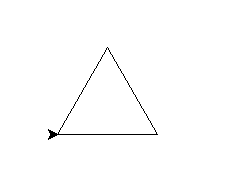
\includegraphics[width=2.0in]{img/triangle}
%    \vspace{-10mm}
    \end{center}
\end{ex}

\begin{ex}[navigate.py] Write a program that takes directions from the command line
    to draw a line. Let the user input ``left'', ``right'', ``forward'', or
    ``stop''. Left and right turn the turtle left or right however many degrees
    are entered, forward moves the turtle forward (however far you wish), and
    stop ends the program. Please check the degrees for errors: they must be
    between 0 and 360 degrees! (Yes, Turtle could handle negative degrees, but
    we would like you to check.)

    Input:

  \begin{verbatimcode}
Please enter a direction: forward
Please enter a direction: left
How many degrees? 45
Please enter a direction: forward
Please enter a direction: left
How many degrees? -1
Invalid number, not moving.
Please enter a direction: left
How many degrees? 45
Please enter a direction: forward
Please enter a direction: forward
Please enter a direction: left
How many degrees? 45
Please enter a direction: left
How many degrees? 45
Please enter a direction: forward
Please enter a direction: right
How many degrees? 45
Please enter a direction: forward
Please enter a direction: stop
  \end{verbatimcode}

    Output:
    \begin{center}
%    \vspace{-5mm}
    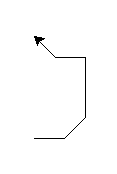
\includegraphics[width=1.0in]{img/navigate}
%    \vspace{-10mm}
  \end{center}

\end{ex}

\newpage
\section{Extra Credit Exercise}
\vspace{-1.5em}
Irrational numbers, like $\pi, \log 2$ or $e$ do not terminate and are not generally easy to compute (unlike $1/9 = 0.1111\dots$, for example.)
In this exercise, you will write a Python script that can calculate the $n^\text{th}$ digit of $\pi$ without having to compute the first $n-1$ digits of $\pi$.

Your program will find the $n^\text{th}$ digit of $\pi$ in hexadecimal base instead of the usual decimal base. For example, here are the first four digits after the decimal of $\pi$: $\pi = 3.14\dots_{10} = 3 \cdot 10^0 + 1 \cdot 10^{-1} + 4 \cdot 10^{-2}$.
In hexadecimal notation, instead of powers of 10, there are powers of 16 and digits go from 0 to A (which represents 10) and on to F (which represents 15) instead of 0 to 9. Here are some examples:
\begin{align*}
1A.0C_{16} &= 1 \cdot {16^2} + 10 \cdot 16^1 + 0 \cdot 16^{-1} + 12 \cdot 16^{-2}
&
1A &= 1 \cdot {16^2} + 10 \cdot 16^1
\end{align*}
\vspace{-1.5em}
$$\pi = 3.243F\dots_{16} = 3 \cdot 16^0 + 2 \cdot 16^{-1} + 4 \cdot 16^{-2} + 3 \cdot 16^{-3}
      + 15 \cdot 16^{-4} + \cdots
$$

The first 30 digits of $\pi$ written in hexadecimal are equal to the first 36 digits of $\pi$ in decimal:
\begin{align*}
\pi &= 3.141592653589793238462643383279502884_{10}\dots
\\
\pi &= 3.243F6A8885A308D313198A2E037073_{16}\dots
\end{align*}

Also, sigma notation is used to represent summations.
Here are some examples:

\vspace{-1.5em}
\begin{align*}
\sum_{i=10}^13 i &= 10 + 11 + 12 + 13
                   &
\sum_{k=1}^4 \frac{16^k}{8k + j} &= \frac{16}{j} + \frac{16^2}{16 + j} + \frac{16^3}{24 + j} + \frac{16^4}{32 + j}
\end{align*}

\begin{extraex}[extra\_credit\_pi.py]
Write a function \pythoninline{digits(n)} that finds the $n^\text{th}$ digit of $\pi$ in hexadecimal.
A variation of the Bailey-Borwein-Plouffe can be used.
The formula relies on a helper function $S$:
\vspace{-1.1em}
\begin{align*}
S(j, n) &= \left(\sum_{k=0}^n \frac{\left(16^{d-k}\right) \text{ mod } (8k + j)}{8k + j} \right) + \sum_{k=d+1}^{100} \frac{16^{d-k}}{8k+j}
\\
\text{$n^\text{th}$ of $\pi$} &= 4S(1, n) - 2S(2, n) - S(5, n) - S(6, n)
\end{align*}

The function $\pythoninline{digits(n)}$ must return a string representing the hexadecimal digits at the $n^\text{th}$ place of $\pi$.
This string can be at most 10 characters in length
(hint, use the function included in the template file: $\pythoninline{decimal_to_hex(s, 10)}$.)
The code used to test this function relies on this name and behavior.
It is highly recommended to use the included function
\pythoninline{expm(b, p, ak)} for efficiently calculating
\begin{center}
$(b^p) \text{ mod } ak =$ \pythoninline{(b ** p) % ak}.
\end{center}

$\pi = 3.243F6A8885A30\dots$ in hexadecimal, so your program's output should be:
\begin{pyconcode}
>>> from extra_nth_pi import digits
>>> digits(0)
243F6A8885
>>> digits(3)
F6A8885A30
>>> digits(1000000)
6C65E52CB4
\end{pyconcode}
\end{extraex}

\pagebreak
\section{Submitting}

You should submit your code as a tarball. It should contain all files
used in the exercises for this lab. The submitted file should be named
\begin{center}
  \texttt{cse107\_firstname\_lastname\_lab2.tar.gz}
\end{center}

\begin{center}
  \textbf{Upload your tarball to Canvas.}
\end{center}

\listexercises
\listextraexercises

\end{document}
